\documentclass[12pt,oneside,openany,letterpaper]{article}


\usepackage{fancyhdr}
\usepackage{helvet}
\usepackage{amsmath}
%\usepackage{graphicx}
\usepackage[pdftex]{graphicx}
\usepackage{psfrag}
\usepackage{setspace}
%\usepackage[hypertex, linktocpage]{hyperref}[2003/11/30]
\usepackage[linktocpage]{hyperref}[2003/11/30]
\usepackage{lscape}
\usepackage{nicefrac}
\usepackage{mathrsfs}
\usepackage{units}
\usepackage{upgreek}
\usepackage{amssymb}
\usepackage{color}
\usepackage{wrapfig}
\usepackage{multirow}
\usepackage{url}
\usepackage{verbatim}
\usepackage{textcomp}
\usepackage{epstopdf}

\onehalfspacing \setlength\textheight{667pt}
\setlength\textwidth{506pt} \setlength\oddsidemargin{-18pt}
\setlength\topmargin{-20pt}
%\setlength\footskip{24pt}
\addtolength\headheight{2.5pt} \addtolength\headsep{-14pt}
%\fancyhead[R]{\includegraphics[height=10.5pt]{ubclogo_bw.eps}\#:  55907968}
%\renewcommand\familydefault{\sfdefault}
\pagestyle{empty}

\newenvironment{packed_enum}{
\begin{enumerate}
  \setlength{\itemsep}{0pt}
  \setlength{\parskip}{0pt}
  \setlength{\parsep}{0pt}
}{\end{enumerate}}

\newenvironment{packed_item}{
\begin{itemize}
  \setlength{\itemsep}{0pt}
  \setlength{\parskip}{0pt}
  \setlength{\parsep}{0pt}
}{\end{itemize}}


\fancyhead[L]{\emph{Introduction to Electronics}}\fancyhead[R]{$LRC$ Transients and Resonance}
\fancyfoot[L]{PHYS 231}\fancyfoot[R]{Experiment 3}
\pagestyle{fancy} \pagenumbering{arabic}

\begin{document}
\thispagestyle{plain}
\begin{center}
{\large{\bf{\fontfamily{phv}\selectfont Physics 231 - Transients in $RC$ Circuits (Exp.~3)}}}
\end{center}

\noindent In this experiment you will be measuring the transient responses of $RC$ circuits, first with the oscilloscope and then using the automatic data storage capability of the Agilent 34401A Digital MultiMetre (DMM). For the final analysis you will perform a linear fit to the data acquired from the DMM.

~


{\bf Part 1 - Rough Measurement of Time Constant with the Oscilloscope}

~

\noindent In the first part of this experiment you will use the oscilloscope to make a quick estimate of the time constant of a series RC circuit.  This part of the lab is designed to take no more than $45$ minutes. The function generator is used to produce a low-frequency square wave signal, repeatedly jumping from zero up to some positive voltage and back to zero.  You should take a minute to think about how low is low enough.  
\begin{figure}[h!]
\begin{center}
\includegraphics[width=.6\textwidth]{figures/Lab3Fig1.pdf}\caption{\label{fig:fig1}The circuit used in part 1 to make a quick estimate of the $RC$ time constant.}
\end{center}
\end{figure}

~

\noindent Set up the circuit shown in Fig.~\ref{fig:fig1}. Measure the capacitor voltage $V_C$ on channel 1 and the output voltage of the function generator, $V_0$, on channel 2 of the oscilloscope. Set the
generator to square wave output to a low frequency since the time constant of this circuit is quite long.  The voltage across capacitor $C$ discharging through a resistor $R$ is given by:
\begin{equation}
V_C(t) = V_C(t=0)e^{-t/\tau},
\end{equation}
where $\tau = RC$ is the time constant. Thus, you should observe an exponentially decaying voltage on channel 1. A quick estimate of the time constant can be made by measuring the time it takes for the voltage across the capacitor to drop to $1/e$ of its initial value at the start of an oscilloscope sweep. Compare the measured time constant with that expected from the component values. Remember, meaningful comparisons require uncertainty estimates.  You should have uncertainties for both the measured and expected values of $\tau$.


\clearpage


{\bf Part 2 - Measurement of the $RC$ Time Constant with the DMM}

~

\noindent Rearrange the circuit as shown below in Fig.~\ref{fig:fig2}. The circuit is designed to have the same $RC$ time constant as in Fig.~\ref{fig:fig1}, but the transient is initiated by disconnecting the voltage
source using the switch.

~

\noindent The DC voltage can be obtained from the function generator by setting the frequency to ``0000'' (decrease the frequency range until only zeros are displayed). The capacitor voltage
should be measured with the HP/Agilent/Keysight DMM.

\begin{figure}[h!]
\begin{center}
\includegraphics[width=.8\textwidth]{figures/Lab3Fig2.pdf}\caption{\label{fig:fig2}The circuit used in part 1 to make a more careful estimate of the $RC$ time constant.}
\end{center}
\end{figure}

\noindent You will find details on programming the DMM on the course website. (First click on the Instrument Specs link and then open “\verb|34401A_Users_Ed7_Online.pdf|”. The
relevant information can be found in Chapter 2.)

~

\noindent The basic idea is to take voltage measurements at equally spaced time intervals, starting at or slightly after the moment you disconnect the voltage source at switch. Since the time constant is faster than the speed at which you have normally taken DC measurements, you will need to take some care to set up the DMM so that it takes data quickly. In the DMM's programming menu you will need to make the following settings:

\begin{packed_item}
\item {\bf Trigger Delay} set to {\bf 0.2~s} (this is the time between data points)
\item {\bf Number of Samples} set to {\bf 20} (the number of data points)
\item {\bf Resolution} set to {\bf "4 digits - Slow"} (needed for speed, the default is 5 digits - slow)
\item {\bf Store Readings} set to {\bf "ON"} (you need to do this before every data set that you collect)
\item {\bf Note: after each one of these changes you must press ENTER in order for the change to be stored in memory}
\end{packed_item}

~

\noindent You will also need to set the DMM's autorange feature to manual in order to block the DMM from trying to change ranges in the middle of your measurement. This means you will have to manually select the voltage range that is suitable for measuring up to $10\rm\ V$.

~

\noindent If everything is set right, you should be able to start collecting data by pressing {\bf Trigger}. When the 20 measurements are complete you can re-enter the menu to observe the measurements under {bf Saved Readings}. Record the measurements in your notebook and use the Jupyter notebook linked on the course website to plot a graph of $\ln V_C$ vs $t$.  You will also fit the data to a straight line (it should be a {\it weighted} linear fit).  Use the slope of the fit and its uncertainty to find $\tau\pm\Delta\tau$.  

~

\noindent Compare the time constants obtained in the two different measurements and explain the difference, if any.  Also, compare the measured time constants to the expected value.

\end{document}
